\chapter{Support Vector Machines}

{\sf Support vector machines (SVM) were a widely used method in 2000s. But it's still a very nice method when you have a small data problem. Let's imagine we have two classes ($+1$ and $-1$) and we have 3 possible hypotheses [pic. 9.1]. The red one is better than others. So SVM maximize the margins -- distances of the closest points of each class. It's mathematically proved that it's an optimal desicion. The bigger the margins then the higher the probability that we are correct on the general set. How do we solve it?}
\begin{figure}[h]
  \centering
  \begin{subfigure}[c]{0.4\linewidth}
    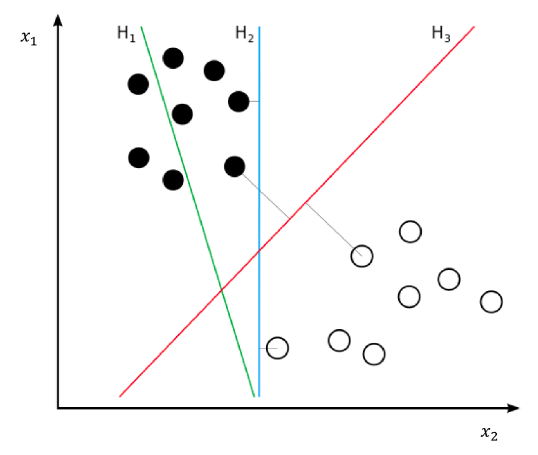
\includegraphics[width=\linewidth]{9a.png}
    \caption*{(9.1) Linear hypotheses}
  \end{subfigure}
  \hspace{2cm}
  \begin{subfigure}[c]{0.35\linewidth}
    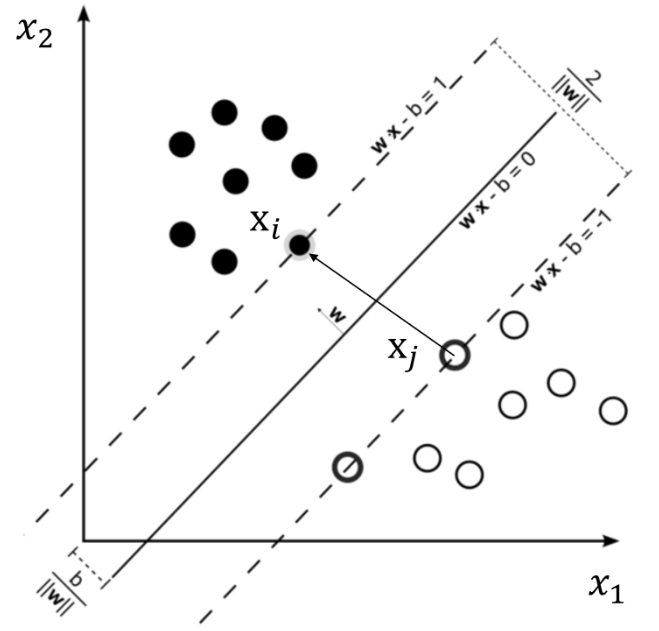
\includegraphics[width=\linewidth]{9b.png}
    \caption*{(9.2) Maximize the margin}
  \end{subfigure}
  \vspace{-0.4cm}
\end{figure}

\section{Linearly Separable Case}
\vspace{-0.6cm}
\subsubsection*{Maximize the margin}

Let's say we have an optimal hyperplane $H$ what defined by a norm vector $w$ [pic. 9.2] (formula for $H$ is $w^Tx-b=0$). $H$ is optimal so the distances from $H$ to $x_j$ (closest point to $H$ from one class) and from $H$ to $x_i$ (closest point from another class) are maximal. The sum of that distances is the result of projecting $\overrightarrow{x_jx_i}$ on $w$ divided by $\|w\|$:
$$\frac{w^T(x_i-x_j)}{\|w\|}$$
what we want to maximize. Also $H$ is on the middle between $x_i$ and $x_j$ (because we want to maximize both distances $x_i$ to $H$ and $x_j$ to $H$). If we multiply $w$ and $b$ by same value, the $H$ will not change, so let's scale $w$ and $b$ such that hyperplane $wx-b=-1$ contains point $x_j$ ($w^Tx_j-b=-1$) and hyperplane $wx-b=1$ contains point $x_i$ ($w^Tx_i-b=1$). So we want to maximize:
$$\frac{w^T(x_i-x_j)}{\|w\|}=\frac{w^Tx_i-b-(w^Tx_j-b)}{\|w\|}=\frac{2}{\|w\|}$$
or, what is equal, minimize $\|w\|=w^Tw$ under $y_k(w^Tx_k-b)\ge 1$ constraints for every point $x_k$ from the dataset. That constraint means that point $x_k$ with $y_k=-1$ is in one subspace (when $w^Tx_k-b\le-1$) and with $y_k=1$ is in the other (when $w^Tx_k-b\ge1$). So this is an optimization task for SVM:
$$\begin{cases}
	\frac{1}{2}w^Tw\to\min, \\
	y_i(w^Tx_i-b)\ge1.
\end{cases}$$
The solution of this quadratic problem is quite easy, but we are going to do it in a complicated way.

\subsubsection*{Karush-Kuhn-Tucker conditions}

So we have an optimisation task (what is called the primal problem):
$$\begin{cases}
	\min\limits_{z}f(z), \\
	g_i(z)\le0, \\
	h_i(z)=0.
\end{cases}$$
If $z^*$ is a local minimum, then there are Lagrangian multipliers $\alpha_i^*$ and $\beta_j^*$ for:
$$\mathcal{L}(z,\alpha,\beta)=f(z)+\sum\limits_{i=1}^{m}\alpha_i g_i(z)+\sum\limits_{j=1}^{n}\beta_jh_j(z)$$
such that (Karush-Kuhn-Tucker conditions):
$$\begin{cases}
	\frac{\partial}{\partial z_i}\mathcal{L}(z^*,\alpha^*,\beta^*)=0, \\
	\frac{\partial}{\partial \beta_i}\mathcal{L}(z^*,\alpha^*,\beta^*)=0, \\
	\alpha_i g_i(z^*)=0, \\
	\alpha_i^*\ge0.
\end{cases}$$
And finding the solution of the primal problem is equal to finding the solution of the dual problem (if both solutions exists):
$$\max\limits_{\alpha,\beta}\min\limits_{z}\mathcal{L}(z,\alpha,\beta),\qquad\alpha\ge0$$
[Важно понимать, что иногда при решении двойственной проблемы удобно пользоваться условиями Karush-Kuhn-Tucker. Мы можем так делать, поскольку решение двойственной задачи является решением исходной, а те условия следуют из существования решения исходной задачи.]

\subsubsection*{Solution of the dual problem}

So if we formulate our SVM task in terms of the primal problem, we will have
$$\begin{cases}
	\frac{1}{2}w^Tw\to\min, \\
	-(y_i(w^Tx_i-b)-1)\le0.
\end{cases}$$
And we get this optimization problem ($z=(w,b)$):
$$\max\limits_{\alpha}\min\limits_{z}\mathcal{L}(\overbrace{w,b}^z,\alpha)=\frac{1}{2}(w^Tw)-\sum\limits_{i=1}^{N}\alpha_i(y_i\big(w^Tx_i-b\big)-1),\qquad\alpha_i\ge0$$
Let's find $q(\alpha)=\min\limits_{w,b}\mathcal{L}(w,b,\alpha)$ [достаточно найти градиенты, поскольку по условию исходной задачи нужные нам $w$ и $b$ существуют]:
$$\begin{cases}
	0=\nabla_w\mathcal{L}(w^*,b^*,\alpha)=w^*-\sum\limits_{i=1}^{N}\alpha_iy_ix_i\Rightarrow w^*=\sum\limits_{i=1}^{N}\alpha_iy_ix_i &  \\
	0=\nabla_b\mathcal{L}(w^*,b^*,\alpha)=\sum\limits_{i=1}^{N}\alpha_iy_i & 
\end{cases}\Longrightarrow$$
$$\Longrightarrow q(\alpha)=\mathcal{L}(w^*,b^*,\alpha)=\frac{1}{2}\big(w^{*^T}w^*\big)-\sum\limits_{i=1}^{N}\alpha_i(y_i\big(w^{*^T}x_i-b^*\big)-1)=$$
$$=\frac{1}{2}\Big(\sum\limits_{i=1}^{N}\alpha_iy_ix_i\Big)^T\Big(\sum\limits_{i=1}^{N}\alpha_iy_ix_i\Big)-\sum\limits_{i=1}^{N}\alpha_i\big(y_i\Big(\Big(\sum\limits_{j=1}^{N}\alpha_jy_jx_j\Big)^Tx_i-b^*\Big)-1\big)=$$
$$=\frac{1}{2}\sum\limits_{i=1}^{N}\sum\limits_{j=1}^{N}y_iy_ja_ia_jx_i^Tx_j-\sum\limits_{i=1}^{N}\sum\limits_{j=1}^{N}y_iy_ja_ia_jx_i^Tx_j+b^*\sum\limits_{i=1}^{N}a_iy_i+\sum\limits_{i=1}^{N}a_i=$$
$$=\sum\limits_{i=1}^{N}a_i-\sum\limits_{i=1}^{N}\sum\limits_{j=1}^{N}y_iy_ja_ia_jx_i^Tx_j$$
And we get quadratic optimization problem under linear constraints:
$$\max\limits_{\alpha}q(\alpha),\qquad\alpha_i\ge0,\qquad 0=\sum\limits_{i=1}^{N}\alpha_iy_i$$
what is efficiently solved by quadratic programming.

\subsubsection*{CVXOPT package}

Our quadratic problem we can solved by CVXOPT package. It solves this kind of tasks:
$$\begin{cases}
	\frac{1}{2}\alpha^TP\alpha+q^T\alpha\to\min,\\
	G\alpha\le h, \\
	A\alpha=b.
\end{cases}$$
In terms of our problem:
$$\begin{cases}
	P_{ij}=y_iy_jx_i^Tx_j, & q_i=-1, \\
	G=-I_N, & h_i = 0, \\
	A=y^T, & b_i = 0.
\end{cases}$$
But why did we use the dual problem? Why we can't solve our task in terms of primal problem by using this package? That's because if we use the dual problem, we will able to use the kernel trick.

\subsubsection*{Support vectors}

So we can find the $w$ parameter of the optimal hyperplane. How to find $b$? Well, we already know from Karush-Kuhn-Tucker conditions that $\alpha_i(y_i(w^Tx_i-b)-1)=0$. For most points $\alpha_i=0$ but there are some points (support vectors) with $\alpha_i>0$. For them $y_i(w^Tx-b)=1$ what helps us find $b$. The support vector exists because we scaled $w$ and $b$.

\pagebreak
\section{Linearly Inseparable Case}
\vspace{-0.6cm}
\subsubsection*{Kernel trick}

If we have linearly inseparable dataset we can made it linearly separable using \hyperlink{new_features}{feature enginering}. It needs to increase dimension of our dataset by adding new features. But we can avoid this, if we use only scalar product in all calculations. We do not need to transition into higher dimensional space but rather only
define a scalar product operation $K$ (kernel) there. Here you can see some kernes:\\
\begin{figure}[h]
  \centering
  \begin{tabular}{ccc}
    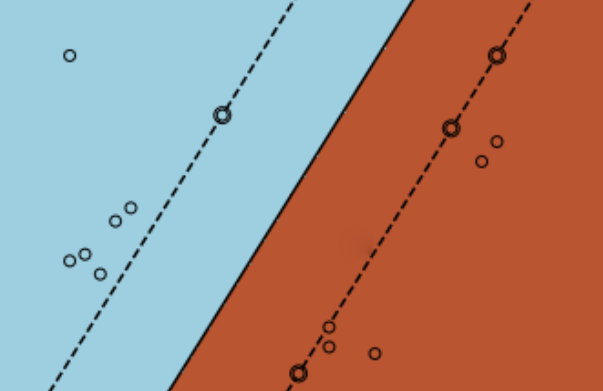
\includegraphics[width=0.25\linewidth]{9c.png} & \hspace{0.5cm}
    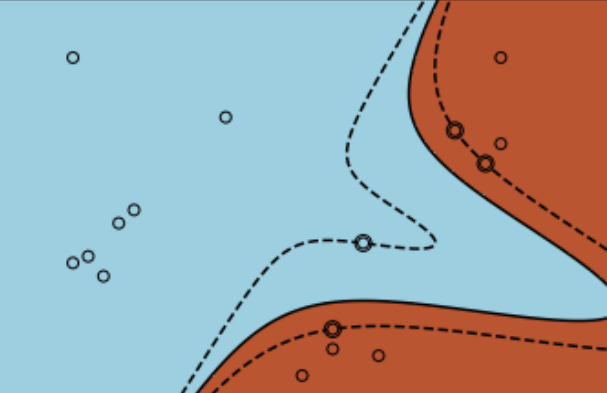
\includegraphics[width=0.25\linewidth]{9d.png} & \hspace{0.5cm}
    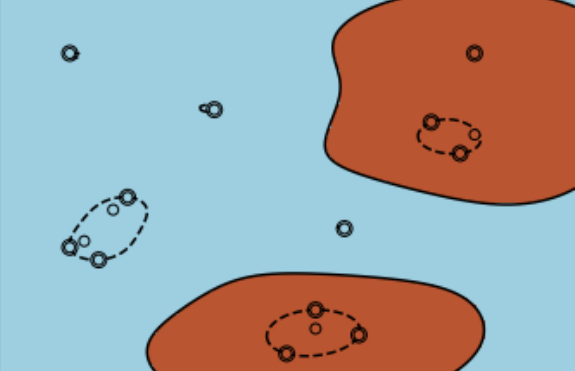
\includegraphics[width=0.25\linewidth]{9e.png} \\
    $\langle x_1,x_2\rangle$ & $(r+\gamma\langle x_1,x_2\rangle)^d$ & $e^{-\gamma|x_1-x_2|^2}$ \\
  \end{tabular}
  \vspace{-0.8cm}
\end{figure}

\subsubsection*{Soft margin}

\begin{wrapfigure}{r}{0.35\linewidth}
  \vspace{-1.4cm}
  \begin{center}
    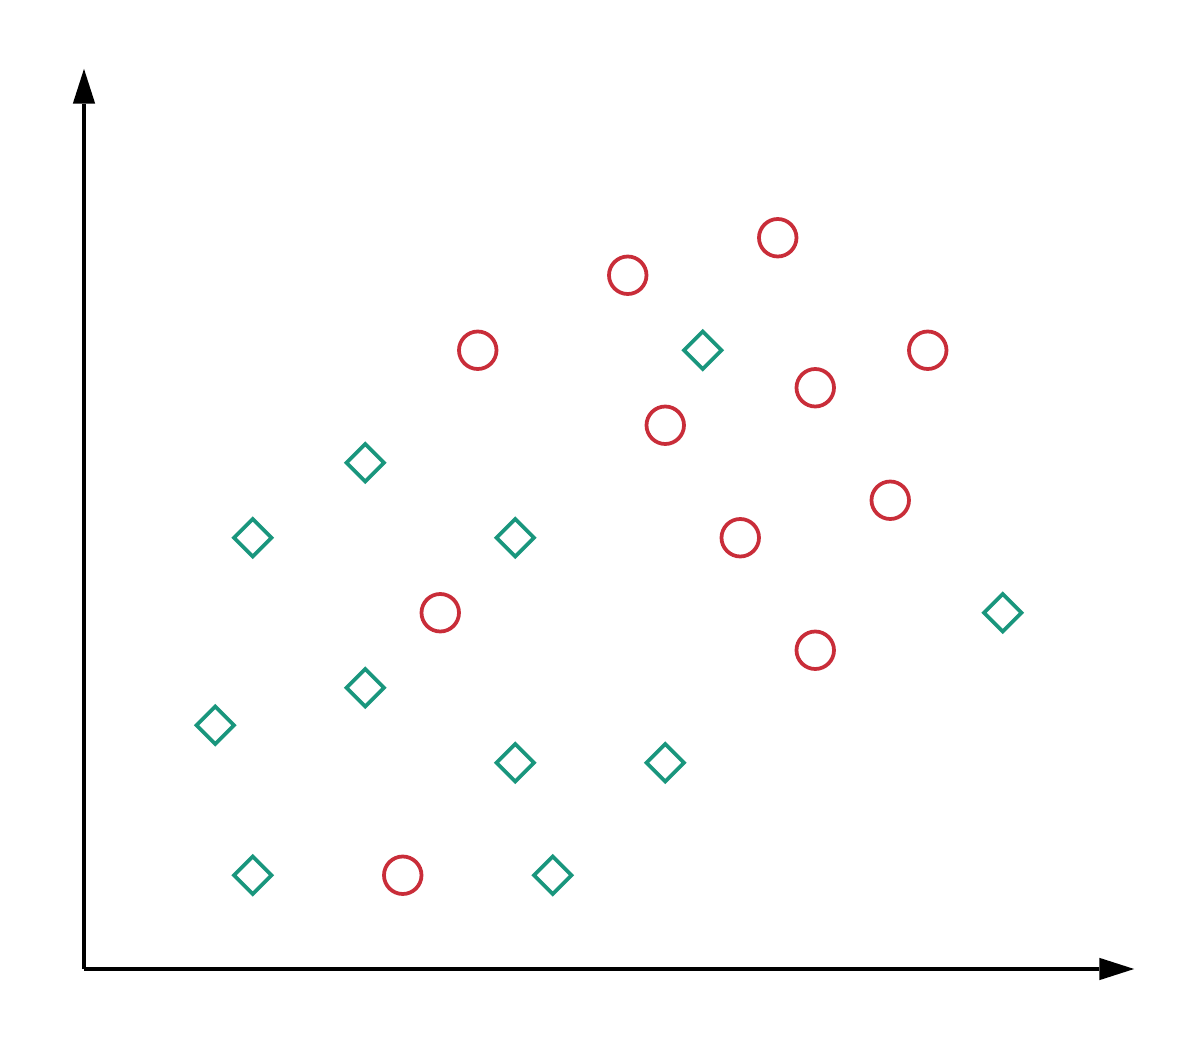
\includegraphics[width=\linewidth]{9f.png}
  \end{center}
  \vspace{-0.6cm}
  \caption*{(9.3) Linear inseparable}
  \vspace{-0.8cm}
\end{wrapfigure}
If we have some bad points [pic. 9.3.] what make our dataset linearly inseparable, we want to skip these points and apply our algorithm for the linearly separable case. This way calls soft margin. So the optimization task for the soft margin looks like this:
$$\begin{cases}
	\frac{1}{2}(w^Tw)+C\sum\limits_{i=1}^{N}\xi_i\to\min, \\
	y_i(w^Tx_i-b)\ge1-\xi_i, \\
	\xi_i\ge0.
\end{cases}$$
$C$ is a some constant. When $C$ is small, the SVM focuses on maximizing the margin, whereas $C$ is large, the focus is more on avoiding missclassification. Also we define variable $\xi_i$ for every point $x_i$; $\xi_i$ is a distance of $x_i$ to the hyperplane $y_i(w^Tx-b)=1$ if $y_i(w^Tx-b)<1$.\\
Otherwise $\xi_i=0$.

\subsubsection*{Dual problem for soft margin}

The dual problem for soft margin is finding the $\max\limits_{\alpha}\min\limits_{z}\mathcal{L}(z,\alpha)$ for $\alpha_i\ge0$, where
$$\mathcal{L}(\overbrace{w,b,\xi}^{z},\underbrace{\bar\alpha,\dot\alpha}_{\alpha})=\frac{1}{2}(w^Tw)+C\sum\limits_{i=1}^{N}\xi_i-\sum\limits_{i=1}^{N}\bar\alpha_i(y_i\big(w^Tx_i-b\big)-1+\xi_i)-\sum\limits_{i=1}^{N}\dot\alpha_i\xi_i=$$
$$=\frac{1}{2}(w^Tw)-\sum\limits_{i=1}^{N}\bar\alpha_i(y_i\big(w^Tx_i-b\big)-1)-\sum\limits_{i=1}^{N}\xi_i(\dot\alpha_i+\bar\alpha_i-C)$$
[Здесь под $\alpha_i$ подразумевается не пара $(\bar\alpha_i,\dot\alpha_i)$, а равенства $\bar\alpha_i = \alpha_i$ и $\dot\alpha_i=\alpha_{i+N}$.]\\
Let's find $q(\alpha)=\min\limits_{z}\mathcal{L}(z,\alpha)$:
$$\begin{cases}
	0=\nabla_w\mathcal{L}(w^*,b^*,\xi^*,\alpha), \\
	0=\nabla_b\mathcal{L}(w^*,b^*,\xi^*,\alpha), \\
	0=\nabla_\xi\mathcal{L}(w^*,b^*,\xi^*,\alpha).
\end{cases}\Longrightarrow
\begin{cases}
	w^*=\sum\limits_{i=1}^{N}\bar\alpha_iy_ix_i, \\
	\sum\limits_{i=1}^{N}\bar\alpha_iy_i=0, \\
	\bar\alpha_i=C-\dot\alpha_i\Rightarrow 0\le\bar\alpha_i\le C.
\end{cases}\Longrightarrow$$
$$\Longrightarrow q(\alpha)=\mathcal{L}(w^*,b^*,\xi^*,\alpha)=\frac{1}{2}\big(w^{*^T}w^*\big)-\sum\limits_{i=1}^{N}\bar\alpha_i(y_i\big(w^{*^T}x_i-b^*\big)-1)-\sum\limits_{i=1}^{N}\xi_i^*(\dot\alpha_i+\bar\alpha_i-C)=$$
$$=\sum\limits_{i=1}^{N}\bar\alpha_i-\frac{1}{2}\sum\limits_{i=1}^{N}\sum\limits_{i=1}^{N}y_iy_j\bar\alpha_i\bar\alpha_jx_i^Tx_j$$
Finally we get this optimization problem:
$$\begin{cases}
	\max_{\alpha}q(\alpha), \\
	0\le\bar\alpha_i\le C, \\
	\sum\limits_{i=1}^{N}\bar\alpha_i=0.
\end{cases}$$

\subsubsection*{Vector types}

We have three vector types:
\begin{enumerate}[label=\arabic*.]
	\item Inside vectors: $\bar\alpha_i$, $\xi_i=0$, $y_i(w^Tx_i-b)\ge1$
	\item Good support vectors: $0<\bar\alpha_i<C$, $\xi_i=0$, $y_i(w^Tx_i-b)=1$
	\item Bad support vectors: $\bar\alpha_i=C$, $\xi_i>0$, $y_i(w^Tx_i-b)\le1$
\end{enumerate}
After finding $\bar\alpha_i$ and $\xi_i$ we can easily find good support vectors. And that vectors helps us find $b$ -- the second parameter of the optimal hyperplane. Also there is no other vector types because of primal and dual problem inequalities and Karush-Kuhn-Tucker conditions.

\subsubsection*{Higher dimensionality and generalization}

Even in linearly separable case you may use the soft margin. It allows to priorotize (by choosing constant $C$): you want to have less bad support vectors or you want to have higher margins. However, we should care how many support vectors we have ($E_{gen}$ is a \hyperlink{gen_error}{generalisation error}):
$$E_{gen}\le\frac{|\{x\colon x \text{ is support vector}\}|}{|\{x\colon x \text{ is training vector}\}|}$$

\section{Multi-class SVM}

[Вы просто сводите к задаче бинарной классификации: сначала отделяете один класс от всех, затем другой и т.д. Тем самым вы получаете для каждого класса свой SVM, который сообщает, принадлежит точка этому классу или нет.]